\documentclass{article}

\usepackage{times}
\usepackage{natbib}
\usepackage{amsmath}
\usepackage[pdftex]{graphicx}
\usepackage{sidecap}
\usepackage{hyperref}
\usepackage{float}
\usepackage{algpseudocode}
\usepackage{algorithm}
\usepackage{subfigure}
\hypersetup{
    colorlinks,%
    citecolor=black,%
    filecolor=black,%
    linkcolor=black,%
    urlcolor=black
}

 

\bibpunct{[}{]}{;}{n}{,}{,}

\newcommand{\BibTeX}{{\sc Bib}\TeX}

\begin{document}
\setlength{\parindent}{0in}%Removing Paragraph Indenting in LaTeX
\author{Behnam Asadi}
\title{An Overview in Fuzzy Logic System and Neuro-Fuzzy System}
\date{\today}
\maketitle
\tableofcontents
%\begin{abstract}
%Abstract Here
%\end{abstract}
%
%{\bf Keywords:} fuzzy systems, fuzzy set, neuro-fuzzy systems, fuzzy logic control, fuzzy inference 

\section{What Is Fuzzy Logic}\label{What Is Fuzzy Logic}
\subsection{Introduction}\label{Introduction}
Fuzzy logic systems have vast number of applications in varied area from house appliance 
such as washing machines, and microwave ovens to digital devices cameras, camcorders and  
industrial process control, medical instrumentation, decision-support systems, and portfolio selection.
What makes the Fuzzy Logic powerful is the fact that most of
human reasoning and concept formation is linked to the use of fuzzy rules. 
\\
Designing system with fuzzy logic control \cite{62215}, \cite{158640}, \cite{52552} is based on experience and it  is an experiential process.\cite{7735}.
\\
Table \ref{table_Fuzzy_Logic_Control_Application_Examples} has listed some industrial application of fuzzy logic with their respective inputs( measurements),outputs and knowledge base \cite{299142}.

\begin{center}
\begin{table}[H]
%\small
\caption{Fuzzy Logic Control Application Examples}
%\begin{tabular}{|l |l |l |l| l | }
\begin{tabular}{| p{.5cm}| p{2cm} | p{2cm} | p{2cm}  |  p{3cm} |}

\hline
  No & APPLICATION & INPUTS & OUTPUTS  &KNOWLEDGE BASE \\
\hline
  1 
  & Tension control of paper rolling machine 
  & Speed sensors (two), tension roller position 
  & Servo drives (one each for feed and roll up)
  & Speed, roller deflection and their differentiation
  \\
\hline
  2 
  & Gas and air supply to boiler 
  & Temperature, oxygen  
  & Air valve, gas valve sensors 
  & optimum combustion
  \\
  \hline
  3 
  & Wire sheath molding m/c 
  & Extruding pressure, speed, resin temperature 
  & Heater, servo motor 
  & Change in temp vs change in pressure
  \\
  \hline
  4
  & Knowledge based molding 
  & Operator  observation re bur, wrap and dent of product   
  & Heater, motor  
  & Inference for optimum molding condition 
  \\
  \hline
  5 
  & Oxygenation of boiler water 
  & Electric conductivity  
  & Oxygen valve
  & pump speed and flow
  \\
  \hline
  6 
  & Peak electric load management  
  & Wattmeter, plant temperature, production schedule 
  & Cut-out circuit breakers (one for brightness, each feeder)  
  & Inferences on estimated electric consumption 
  \\
  \hline
  7 
  & Vacuum tank pressure  stabilization  
  & Tank pressure, pump pressure 
  & Pump speed 
  & Inference on tank and pump characteristics
  \\
  \hline
  8 
  & High precision grinding  
  & Grinder motor current and size measurement 
  & Over-ride signal to Numerical Control 
  & Fuzzy profile interpolation 
  \\
  \hline
  9
  & Food juice blending 
  & Sugar densitometer 
  & Pump motors' speed 
  & Inference on mixing curve
  \\
  \hline            
  10 
  & spray painter  
  & Temperature, paint flow, viscosity, thickness 
  & Flow rate signal to control loop 
  & Viscosity vs temperature
  \\
  \hline            
\end{tabular}
\label{table_Fuzzy_Logic_Control_Application_Examples}
\end{table}
\end{center}



\subsection{Why Use Fuzzy Logic}\label{Why_Use_Fuzzy_Logic}


There are several advantageous for using fuzzy logic, here we have listed some of them in brief: 
\citep{Fuzzy_Logic_Toolbox_For_Use_with_MATLAB}
\begin{itemize}
\item It is easy to understand.
\item It is intuitive and based on natural language. 
\item It can be built on top of the experience of experts.
\item It is tolerant in confronting with unaccurate data.
\item Fuzzy logic has flexibility.
\item It is able to model linear and nonlinear problem with arbitrary complexity.

\end{itemize}
\subsection{When to Use Fuzzy Logic Control}\label{When_to_Use_Fuzzy_Logic_Control}
Table \ref{table_Fuzzy_Logic_Control_Application_Examples} illustrates the application example where 
fuzzy logic could be successfully utilized. Here we have summarized conditions and indicators 
where it is applicable to use fuzzy logic\citep{299142} :

\begin{itemize}
\item The process and plant are complex and difficult to control.
\item System operation that depends on operator skill/knowledge and attention.
\item One parameter of the process affects another parameter. 
\item Process that can be modeled linguistically, and not mathematically. 
\item The possibility of expanding products performance and quality.

\end{itemize}
\subsection{When Not to Use Fuzzy Logic}\label{When_Not_to_Use_Fuzzy_Logic}


Fuzzy logic is very robust, convenient and flexible but it is not solution for all problems. If already a simpler solution already exists, use it\citep{Fuzzy_Logic_Toolbox_For_Use_with_MATLAB}.

G. Chen and G. Kairys \cite{299142}  have listed the type of problems which is not recommended to be solved by fuzzy logic: 
\begin{itemize}
\item If the process/plant is strictly linear, or if PID (proportional–integral–derivative) loop control does an adequate job.
\item If high speed is required and fuzzy control rules may be extensive.
\item Value output for fuzzy logic control does not approach final position asymptotically.

\end{itemize}



\subsection{Fuzzy vs. Non-Fuzzy Example}\label{Fuzzy_vs._Non-Fuzzy_Example}
In this section we compare a fuzzy and a non-fuzzy approach for 
solving the problem "right" amount to tip waitperson in restaurant.
This example was taken from the book \textit{Fuzzy Logic Toolbox For Use with MATLAB}  \citep{Fuzzy_Logic_Toolbox_For_Use_with_MATLAB}
and we will use this example and respective images of that example from the mentioned book in the following sections.
\\
\\
$\mathbf{Tipping Problem} $. Assume that the quality of service at a restaurant is given a number between 0 and 10 where 10 is excellent, what should the tip be?

\subsubsection{The Non-Fuzzy Approach}
One simple approach might be tip $\mathit{15\% } $ of the total bill.
but that doesn't really take into account the quality of the service, 
so a more advance solution might be:\\
\begin{center} 
$tip=0.20/10*service+0.05$ 
\end{center}

The model seems fine but if we want the tip, reflects the quality of the food
as well, a new model might needed:\\
\begin{center} 
$tip = 0.20/20*(service+food)+0.05$ 
\end{center}


Suppose you want the service to be a more important
factor than the food quality. Let's say that the service will account for 80% of
the overall tipping "grade" and the food will make up the other $20\%$.\\
A new model seems work better:\\

$servRatio=0.8$
\begin{center} 
$tip=servRatio*(0.20/10*service+0.05) +(servRatio)*(0.20/10*food+0.05);$
\end{center}

\begin{figure}[H]
\begin{center}
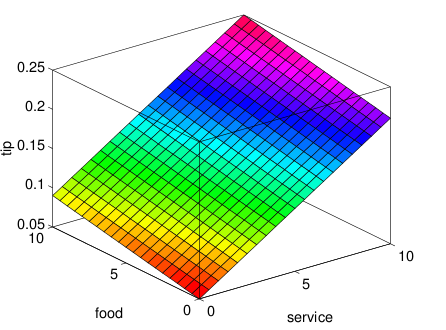
\includegraphics[scale=0.3]{./images/non-fuzzy_linear_tip.png}
\caption{A non-fuzzy linear model for paying tip.}
\label{non-fuzzy_linear_tip}
\end{center}
\end{figure}


The response is still somehow too uniformly linear. Suppose you want more of
a flat response in the middle, i.e., you want to give a $15\%$ tip in general, and
will depart from this plateau only if the service is exceptionally good or bad.
This, in turn, means that those nice linear mappings no longer apply.


$servRatio=0.8$
\begin{algorithmic}

\If {$service \leq 3$}
	
	\State $tip=((0.10/3)*service+0.05)*servRatio +(1 servRatio)*(0.20/10*food+0.05)$

\ElsIf {$service \leq 7$}
     \State $tip=(0.15)*servRatio +(servRatio)*(0.20/10*food+0.05)$
\Else 
	\State  $tip=((0.10/3)*(service 7)+0.15)*servRatio + (servRatio)*(0.20/10*food+0.05)$
   
\EndIf
\end{algorithmic}

\begin{figure}[H]
\begin{center}
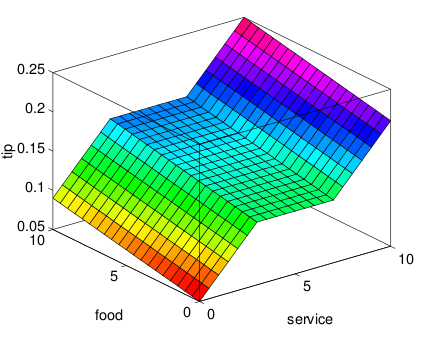
\includegraphics[scale=0.3]{./images/non-fuzzy_non_linear_tip.png}
\caption{A non-fuzzy non linear model for paying tip.}
\label{non-fuzzy_linear_tip}
\end{center}
\end{figure}

The new model looks perfect, but the function is very complicated and it's definitely not easy to modify this
code in the future. Moreover, it's even less apparent how the algorithm works
to someone who didn't witness the original design process.


%sophisticated 
\subsubsection{Fuzzy Approach}
If we express linguistically what is determining our tip payment and make a list of what really matters, we can summarized it in the following list:
\begin{itemize}
\item If service is poor or the food is rancid, then tip is cheap
\item If service is good, then tip is average
\item If service is excellent or food is delicious, then tip is generous
\end{itemize}
Now the important question is what does the "average" mean mathematically in "If service is good, then tip is average" or how can we combine these rule to determine the payment.
These conditional sentences are fuzzy approach for our problem, of course it is not completed yet.
In the following sections we would try to answer these question and complete our fuzzy inference system. 
but before that we need to know the theory and fundamental of fuzzy logic.


\section{Fundamental and Theory of Fuzzy Logic}\label{Fundamental_and_Theory_of_Fuzzy_Logic}
\subsection{Fuzzy Sets}
Fuzzy logic starts with the concept of a fuzzy set. A fuzzy set is a set without a crisp, clearly defined boundary. It can contain elements with only a partial degree of membership.\cite{Fuzzy_Logic_Toolbox_For_Use_with_MATLAB}



\subsection{Definition}
Let X be a space of points( points) with a generic element X denoted by x, Thus $\mathit{X=\{x\}}$.
\\
A $\mathit{fuzzy set(class)} A $  in $\mathit{X}$ is characterized by a $\mathit{membership}$ function $f_{A}(x)$
which associate with each point in X a real number in the interval [0,1], with the value of $f_{A}(x)$
at x representing "the grade of membership" of x in A and 
$\mathit{X}$ is called the universe

\cite{Zadeh1965},\cite{Introduction_to_Fuzzy_Logic_using_MATLAB}.


\subsection{Membership Functions}
A  $\mathit{membership}$ function $\mathit{(MF)}$ is a function that defines how each point in the input
space is mapped to a membership value (or degree of membership) between 0 and 1.\\
$\mu_{A}: X \rightarrow [0, 1]$.

Variety of membership function exist and could be used in fuzzy logic system, figure \ref{Common_membership_functions_in_Matlab} illustrates the most common membership function widely used and their respective function name in Matlab\texttrademark toolbox:



\begin{figure}[H]
\centering
\subfigure[trimf]
{
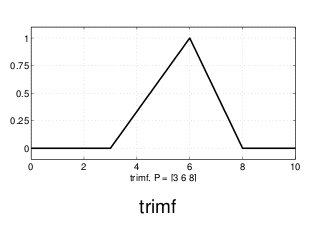
\includegraphics[width=0.3\textwidth]{./images/trimf.png}
\label{fig:trimf}
}
\subfigure[trapmf]
{
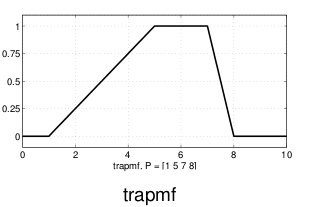
\includegraphics[width=0.3\textwidth]{./images/trapmf.png}
\label{fig:trapmf}
}
\subfigure[gaussmf]
{
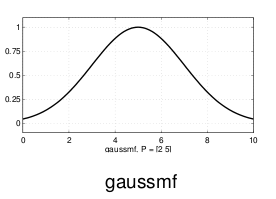
\includegraphics[width=0.3\textwidth]{./images/gaussmf.png}
\label{fig:gaussmf}
}
\label{fig:subfigureExample1}


\subfigure[gauss2mf]
{
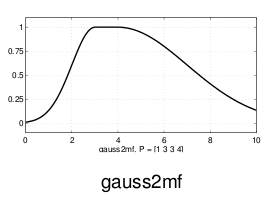
\includegraphics[width=0.3\textwidth]{./images/gauss2mf.png}
\label{fig:gauss2mf}
}
\subfigure[dsigmf]
{
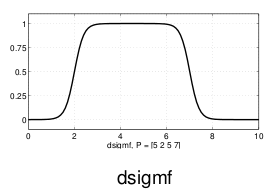
\includegraphics[width=0.3\textwidth]{./images/dsigmf.png}
\label{fig:dsigmf}
}
\subfigure[sigmf]
{
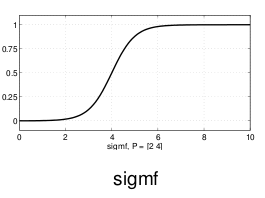
\includegraphics[width=0.3\textwidth]{./images/sigmf.png}
\label{fig:sigmf}
}
\label{fig:subfigureExample2}




\subfigure[psigmf]
{
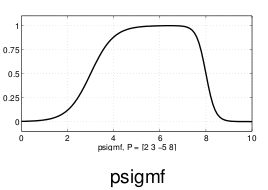
\includegraphics[width=0.3\textwidth]{./images/psigmf.png}
\label{fig:psigmf}
}
\subfigure[zmf]
{
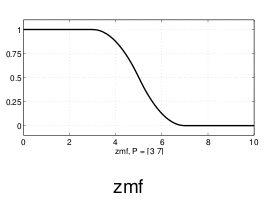
\includegraphics[width=0.3\textwidth]{./images/zmf.png}
\label{fig:zmf}
}
\subfigure[pimf]
{
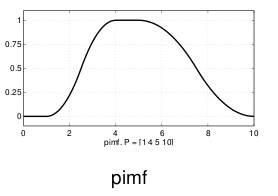
\includegraphics[width=0.3\textwidth]{./images/pimf.png}
\label{fig:pimf}
}
\label{fig:subfigureExample3}




\subfigure[smf]
{
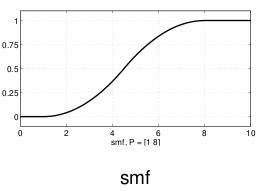
\includegraphics[width=0.3\textwidth]{./images/smf.png}
\label{fig:smf}
}
\subfigure[gbellmf]
{
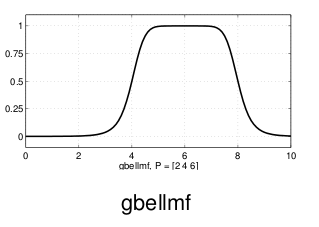
\includegraphics[width=0.3\textwidth]{./images/gbellmf.png}
\label{fig:gbellmf}
}
\caption[Common Membership Functions]

{
Common membership functions in Matlab with their respective function name and parameters.
\label{Common_membership_functions_in_Matlab}
\cite{Fuzzy_Logic_Toolbox_For_Use_with_MATLAB}
}
\end{figure}



\subsection{Fuzzy Set Operations}
Considering three fuzzy sets $\mathit{A}$,$\mathit{B}$ and $\mathit{C}$ on the universe $\mathit{X}$. For a given element $\mathit{x}$ of the universe, the following function theoretic operations for the set theoretic operations unions, intersection and complement are defined for
$\mathit{A}$,$\mathit{B}$ and $\mathit{C}$ on $\mathit{X}$

Union:
\\
\\
$\mu_{A \cup B}  (x)= \mu_{A}(x) \vee  \mu_{B}(x).$ 
\\
\\
Intersection:
\\
\\
$\mu_{A \cap B}  (x)= \mu_{A}(x) \wedge  \mu_{B}(x).$ 
\\
\\
Complement:
\\
\\
$\mu_{\bar{A}}(x)= 1 -  \mu_{A}(x).$ 
%\subsection{Properties of Fuzzy Sets}
%Commutativity:
%Associativity:
%Distributivity:
%Idempotency:
%Identity:
%Transtivity:
%Involution:

\subsection{Logical Operations in Fuzzy Logic}
Fuzzy logical reasoning is a superset of standard Boolean logic. If we use the fuzzy values at their extremes of 1 (completely true), and 0 (completely false), we again would have standard logical operations.




In fuzzy logic the input value can be any real number  between 0 and 1, so we have to find 
a function that preserve the results of the $AND$ and $OR$.

One answer is the  $min$ operator. That resolves the statement, \textbf{A  $AND$ B },
(where A and B are limited to the range between zero and one), by using the function $min(A,B)$.
Using the same reasoning, we can replace the OR operation with the max
function, so that \textbf{A  $OR$ B} becomes equivalent to $max(A,B)$. Finally, the
operation $NOT$ \textbf{A} becomes equivalent to the operation $1 - A$ 
\citep{Fuzzy_Logic_Toolbox_For_Use_with_MATLAB}.
%\citep[p.~12]


\subsection{Conditional Statement in Fuzzy Logic}

A single fuzzy if-then rule assumes the form 
\begin{algorithmic}
\If {$x \; is \; A $}
    \State $y \;is\; B$
\EndIf
\end{algorithmic}

%Spaces in the math-environment can be produced using:
%
%    \; for a thick space,
%    \: for a medium space,
%    \, for a thin space and
%    \! for a negative thin space.
where A and B are linguistic values defined by fuzzy sets on the ranges (universes of discourse) X and Y, respectively.\\
Fuzzy sets and fuzzy operators are the subjects and verbs of fuzzy logic. 
The if-part of the rule is called the $antecedent$ or $premise$, while the then-part of the rule is called
the $consequent$ or $conclusion$.
Interpreting if-then rules is a three-part process. This process can be explained as following:
\begin{itemize}
\item \textit{Fuzzify inputs} 
Resolve all fuzzy statements in the antecedent to a degree of
membership between 0 and 1. If there is only one part to the antecedent, this
is the degree of support for the rule.
\item \textit{Apply fuzzy operator to multiple part antecedents:}
If there are multiple parts
to the antecedent, apply fuzzy logic operators and resolve the antecedent to
a single number between 0 and 1. This is the degree of support for the rule.

\item \textit{Apply implication method:}Use the degree of support for the entire rule to
shape the output fuzzy set. The consequent of a fuzzy rule assigns an entire
fuzzy set to the output. This fuzzy set is represented by a membership
function that is chosen to indicate the qualities of the consequent. If the
antecedent is only partially true, (i.e., is assigned a value less than 1), then
the output fuzzy set is truncated according to the implication method.

\end{itemize}

 
In general, one rule by itself doesn't do much good.There should be two or
more rules so they can play off each other. The output of each rule is a fuzzy set
and in the case that there are more than one rule outputs are aggregated into a single output
fuzzy set. This process will be explained in the section \ref{aggregation}.





\subsection{Defuzzification}
Defuzzification process is the inverse function of fuzzification.
The input for the defuzzification process is a fuzzy set (or if we have more than one rule, the aggregated output of all rules ) and the output is a single number. 
There are several methods of defuzzification\cite{Defuzzification_criteria_and_classification}:

\begin{itemize}\label{list_of_possible_defuzzification}
\item AI (adaptive integration)
\item BADD (basic defuzzification distributions)
\item CDD (constraint decision defuzzification)
\item COA (center of area)
\item COG (center of gravity)
\item ECOA (extended center of area)
\item FCD (fuzzy clustering defuzzification)
\item FM (fuzzy mean)
\item FOM (first of maximum)
\item GLSD (generalized level set defuzzification)
\item ICOG (indexed center of gravity)
\item IV (influence value)
\item LOM (last of maximum)
\item MeOM (mean of maxima)
\item MOM (middle of maximum)
\item WFM (weighted fuzzy mean)
\end{itemize}




\section{Fuzzy Inference Systems}\label{Fuzzy_Inference_Systems}
Fuzzy inference system (FIS) is  the process of using fuzzy logic to formulate  mapping  input to an output.
Fuzzy inference systems have been used for various applications including
data classification, automatic control, computer vision, decision analysis and expert systems.
Because of that fuzzy inference systems have different names  and known as fuzzy expert system,
fuzzy associative memory, fuzzy rule-based systems, and fuzzy model 
\cite{Introduction_to_Fuzzy_Logic_using_MATLAB},\cite{Fuzzy_Logic_Toolbox_For_Use_with_MATLAB}.



This process inference requires all of the previously steps described so far:
membership functions, fuzzy logic operators, and if-then rules.
There are mainly two types of fuzzy inference systems\cite{A_Computational_Approach_to_Learning_and_Machine_Intelligence}:

\begin{itemize}
\item  \textbf{\emph{ Mamdani FIS}}\cite{MamdaniA75} 
\item \textbf{\emph{ Sugeno FIS}} \cite{Industrial_Applications_of_Fuzzy_Control}. 
\end{itemize}
These two vary somewhat in the way outputs are determined.





\subsection{Mamdani Fuzzy Inference System}

Mamdani’s fuzzy inference method was one the first control systems built by Ebrahim Mamdani
in 1975 to control a steam engine and boiler by synthesizing a set of linguistic
control rules. These rules obtained from experienced human operators \cite{MamdaniA75}.
In Mamdani type FIS, the output membership function is a fuzzy set.



After the aggregation, for each output variable there is a fuzzy set which should defuzzified . It is possible to use a single spike as the output membership function.
Later approach is called \emph{singleton} output membership function. 


\subsection{Sugeno Fuzzy Inference System}


Sugeno FIS was proposed  in 1985  \cite{Industrial_Applications_of_Fuzzy_Control}
by Takagi Sugeno Kang. Sugeno type FIS is similar to the Mamdani type FIS. The first two parts of the fuzzy inference process, fuzzifying the inputs and applying the fuzzy operator, are exactly the same.
The main difference between Mamdani and Sugeno is the output membership function.
There is no fuzzy set in output of Sugeno and output membership functions are either linear or constant.

A typical rule in a Sugeno type FIS is in the form of:
\\
\\
If $First Input = x$ and $Second Input = y$, then Output is $z = ax + by + c$.

If $(a=b =0)$, the output level z is a constant. It is called zero-order Sugeno model.

The final output of the system would be weighted average of all rule outputs:
\\
\\
Final Output=$\frac{ \sum_{i=1}^{N} W_{i}Z_{i}  }{ \sum_{i=1}^{N} W_{i} } $
\\
\\
Where $N$ is total number of outputs and $W_{i}$ is weight of $i_{th}$ output.
In general, Sugeno-type systems can be used when output is linear or constant. 
 

%\begin{figure}[H]
%\begin{center}
%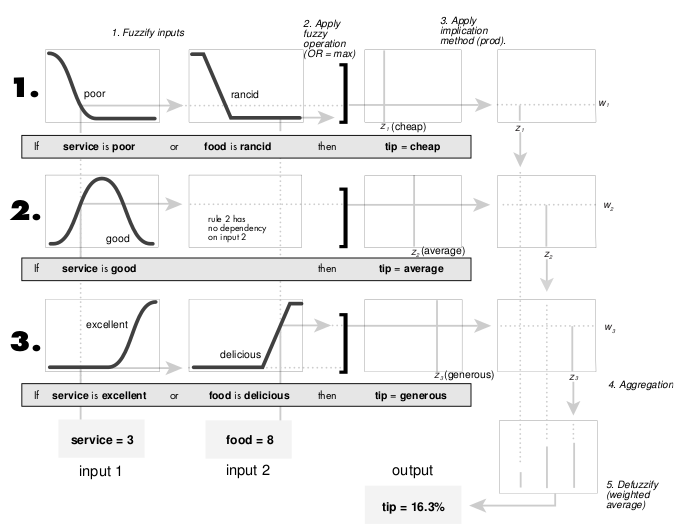
\includegraphics[scale=0.6]{./images/sugeno_paying_tip.png}
%\caption{Fuzzy tipping model expressed with Sugeno type FIS.}
%\label{sugeno-fis}
%\end{center}
%\end{figure}
\subsection{Comparison of Sugeno and Mamdani FIS}
Each one of these fuzzy inferences has it own applications and advantageous and that could be summarized as below\citep{Fuzzy_Logic_Toolbox_For_Use_with_MATLAB}:
\subsubsection{Advantages of the Sugeno Method}
\begin{itemize}
\item It works very good with linear system like PID controller.
\item From computational view it is cheaper in comparison with Mamdani type.
\item It would guarantee that output surface is continuous.
\item For mathematical analysis it suits better.
\end{itemize}

\subsubsection{Advantages of the Mamdani Method}
\begin{itemize}
\item It has been widespread accepted widely used.
\item In comparison with Sugeno It is more intuitive.
\item It's well-suited to human input.
\end{itemize}

\subsection{Fuzzy Inference System for Right Amount of Tips Problem}
In this part we would describe parts of a FIS for right amount of tip, discussed in previous section.
Our system has two input, three rule tipping and one output.
\begin{figure}[H]
\begin{center}
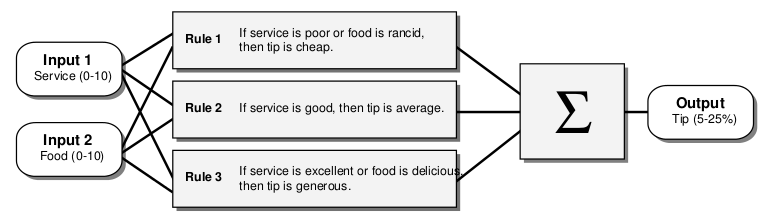
\includegraphics[scale=0.5]{./images/fis_paying_tip.png}
\caption{Problem of paying tips with inputs, rules and outputs.}
\label{fis_paying_tip}
\end{center}
\end{figure}



\begin{itemize}
\item \textbf{Fuzzify Inputs}\\ 
In FIS, the first step is to get the inputs and with membership function determine how well they 
belong to each of the fuzzy sets.

The output is a fuzzy degree of membership in the qualifying linguistic set. 



For instance in our given problem, The first input is "Food", and we want to know
to what extent is the food really delicious with the given value of 8.
by applying membership function we would get, 0.7, so the degree of membership for 
our given input, 8  is 0.7.
\begin{figure}[H]
\begin{center}
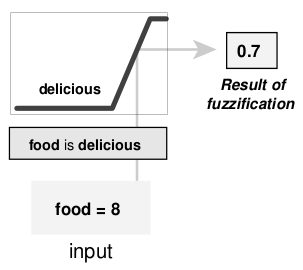
\includegraphics[scale=0.5]{./images/fuzzify.png}
\caption{Fuzzifying Inputs.}
\label{Fuzzify}
\end{center}
\end{figure}


\item \textbf{Apply Fuzzy Operator}\\
Once the inputs have been fuzzified, we know the degree to which each part of
the antecedent has been satisfied for each rule. If the antecedent of a given rule
has more than one part, the fuzzy operator is applied to obtain one number that
represents the result of the antecedent for that rule. This number will then be
applied to the output function. The input to the fuzzy operator is two or more
membership values from fuzzified input variables. The output is a single truth
value.

\begin{figure}[H]
\begin{center}
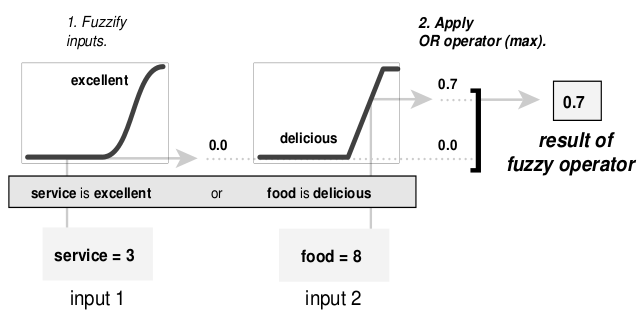
\includegraphics[scale=0.5]{./images/applying_fuzzy_operator.png}
\caption{Applying Fuzzy Operator.}
\label{Apply Fuzzy Operator}
\end{center}
\end{figure}
 

\item \textbf{Apply Implication Method}

Each rule has a weight which shows the relative importance of that rule in comparison with other rule and it is a number between 0 and 1.
This weight is applied to number given by the antecedent.
After proper weighting has been assigned to each rule then implication method can be done.
The input for the implication process is a single number given by the antecedent, and the output is a fuzzy set.
Two method might be used for this step,  "minimum", which truncates the output fuzzy set, and "product", which scales the output fuzzy set. Here we have applied "minimum" method in our implication process for our paying tip rules.


\begin{figure}[H]
\begin{center}
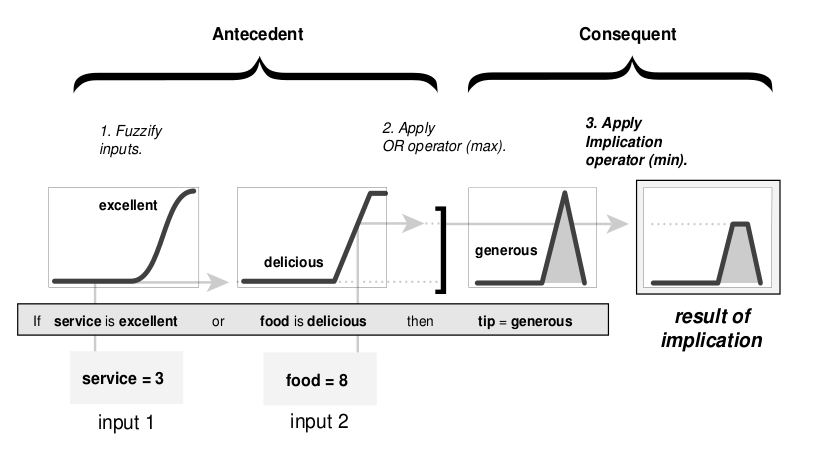
\includegraphics[scale=0.5]{./images/applying_implication_method.png}
\caption{Applying Implication Method.}
\label{Apply Implication Method}
\end{center}
\end{figure}

\item \textbf{Aggregate All Outputs}\label{aggregation}
Since the decisions that should be made by FIS is based on testing all rules and the output of each rule is a fuzzy set, we must combine these fuzzy set into one single set.
The purpose of aggregation is to make such set.


Because the aggregation method is commutative one, then the order of executing rules is not important.
Three methods are used for aggregation:
\begin{itemize}
\item Taking maximum each rule's output set.
\item Probabilistic OR of each rule's output set.
\item Summing each rule's output set.
\end{itemize}

Here we have used maximum function and we took the maximum each rules.
   
\begin{figure}[H]
\begin{center}
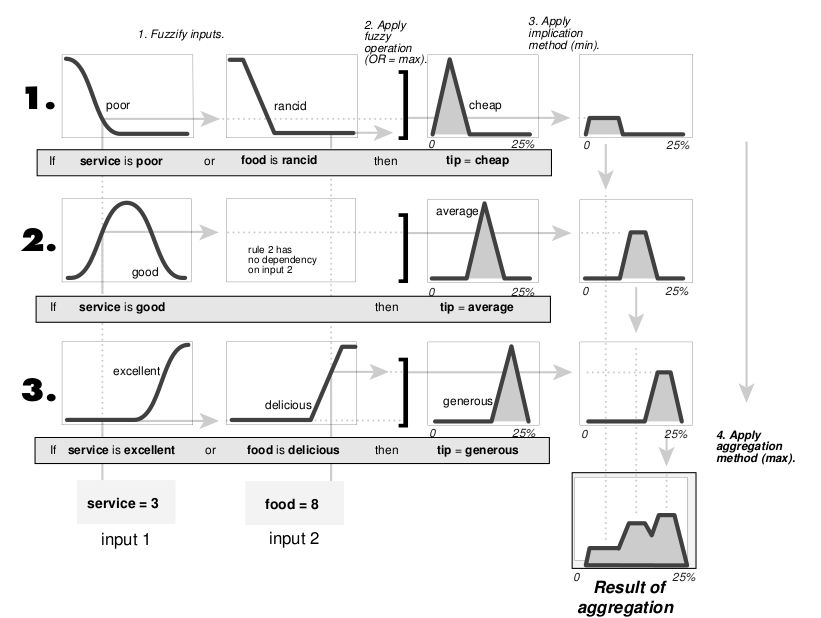
\includegraphics[scale=0.5]{./images/aggregating_all_outputs.png}
\caption{Aggregating All Outputs.}
\label{Aggregating All Outputs}
\end{center}
\end{figure}

\item \textbf{Defuzzify}

The input for the defuzzification is a fuzzy set obtained from aggregation of all the rules
and the output is a single number.

The most popular method for defuzzification is the centroid calculation,
which returns the center of area under the curve \citep{Fuzzy_Logic_Toolbox_For_Use_with_MATLAB}. List of possible defuzzification methods listed in \ref{list_of_possible_defuzzification}




\begin{figure}[H]
\begin{center}
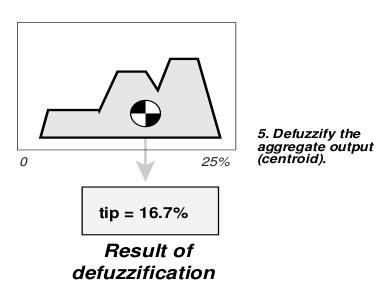
\includegraphics[scale=0.5]{./images/defuzzify.png}
\caption{Defuzzifying.}
\label{Defuzzify}
\end{center}
\end{figure}



\item \textbf{Full FIS for Paying Tips Problem}
Figure \ref{full_FIS_for_paying_tips_problem} illustrates the complete FIS with inputs and respective output.
\begin{figure}[H]
\begin{center}
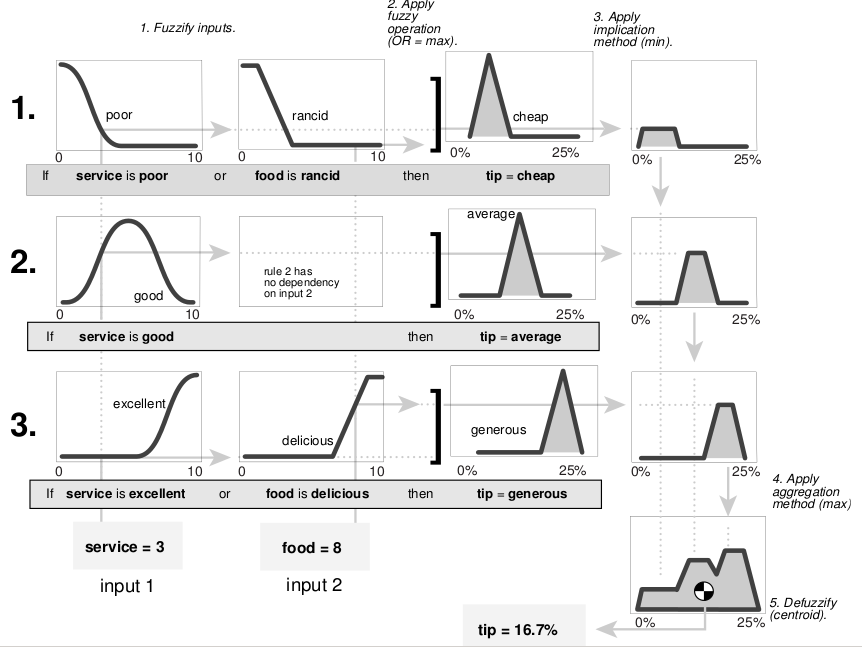
\includegraphics[scale=0.5]{./images/full_FIS_for_paying_tips_problem.png}
\caption{Full FIS for Paying Tips Problem.}
\label{full_FIS_for_paying_tips_problem}
\end{center}
\end{figure}


\end{itemize}






\section{Adaptive Neuro-Fuzzy Inference System }\label{Adaptive_Neuro-Fuzzy_Inference_System}

In the fuzzy inference system that we've seen so far have the below structure and input output flow respectively : 
\begin{itemize}
\item There is a model that maps input to input membership functions.
\item Input membership function to rules
\item From rules to a set of output characteristics.
\item Output characteristics to output membership functions.
\item Finally from membership function to a single-valued output or a decision associated with the output.
\end{itemize}

So far membership functions was chosen arbitrarily. There are limitation with this approach:
\begin{itemize}
\item No standard methods exist for transforming human knowledge or experience into the rule base and database of a fuzzy inference system.
\item There is a need for effective methods for tuning the membership functions to minimize the
output error or maximize performance index.
\end{itemize}
The shape of the membership functions depends on parameters, and changing these parameters will change the shape of the membership function. We are looking for a way so membership function parameters can be chosen automatically. This could be achieved  by using ANFIS (adaptive-network-based fuzzy inference system). 
It was first time proposed and developed by Jyh-Shing Roger Jang \cite{ANFIS_adaptive-network-based_fuzzy_inference_system}.
\\
The basic idea behind ANFIS is learning membership function parameters from a collection of input/output data.
ANFIS uses Artificial Neural Network to learn theses parameters.
%\subsection{Limitations of ANFIS}
%
%ANFIS only works with Sugeno-type systems fuzzy inference systems and following properties must satisfied:
%\begin{itemize}
%\item It must be first or zeroth order Sugeno-type systems.
%\item Output must be a single output, obtained from weighted average defuzzification of all
%output membership functions and theses membership functions must be from the same type or linear or constant.
%\item Number of output membership functions must be equal to the number of rules.
%\item Have unity weight for each rule
%\end{itemize}

\section{Conclusion and Summary}
In this paper we introduced fuzzy logic in \ref{Introduction} and we count the advantages of that in \ref{Why_Use_Fuzzy_Logic}. We gave some example of using fuzzy logic in different application domains with their respective inputs and outputs in table \ref{table_Fuzzy_Logic_Control_Application_Examples}.
In \ref{When_to_Use_Fuzzy_Logic_Control} and \ref{When_Not_to_Use_Fuzzy_Logic} we discussed when should we use fuzzy logic and when we shouldn't.
Then we introduce a problem(right amount of tip) and we gave fuzzy and non fuzzy solution for that
in \ref{Fuzzy_vs._Non-Fuzzy_Example}.
In section \ref{Fundamental_and_Theory_of_Fuzzy_Logic} we formally defined fuzzy sets, membership functions,
fuzzy set operations, logical operations, conditional statement and defuzzification.
In section \ref{Fuzzy_Inference_Systems} we introduced FIS (Fuzzy Inference Systems) and two main FIS, namely Mamdani Fuzzy Inference System and Sugeno Fuzzy Inference System
.We compared them and we counted the advantages of each one and in the following 
we made a FIS for our problem "right amount of tips".
In section \ref{Adaptive_Neuro-Fuzzy_Inference_System} we talked ANFIS in brief and why it is needed.
\\
All in all, fuzzy logic is a widely used method for different applications
because of its easiness, robustness, flexibility, being intuitive and  capable of handling nonlinear problem with arbitrary complexity. 
Although fuzzy logic is very powerful but it is  not a \textit{cure-all} for all problems and some criteria which discussed in \ref{When_Not_to_Use_Fuzzy_Logic} should taken to account before applying that.
\\
Two mainly FIS type, Mamdani and Sugeno, each one is designed for specified application and they have their advantages and disadvantage and one before selecting any of them should consider the type of output which is need.
\\Selecting proper membership function and its parameters needs expert domain knowledge but ANFIS can 
help us to find proper value for the parameters of membership functions, but it still own limitations.  

\section{References }

%\bibliographystyle{plainnat}
\bibliographystyle{ieeetr}
\bibliography{references}

\end{document}
